\documentclass[11pt,a4paper]{article}


\usepackage[margin=1in]{geometry}
\usepackage{microtype}
\usepackage{graphicx}
\usepackage{amsmath,booktabs,hyperref,siunitx}
\usepackage{subcaption}
\usepackage{float}
\usepackage[section]{placeins} 

% --- Header / footer ---
\usepackage{fancyhdr}
\setlength{\headheight}{14pt}
\newcommand{\collegename}{\textbf{UBT}} 
\pagestyle{fancy}
\fancyhf{}
\fancyhead[L]{\collegename}
\fancyhead[R]{\textbf{AI Techniques Lab}}
\fancyfoot[C]{\thepage}
\renewcommand{\headrulewidth}{0.4pt}
\renewcommand{\footrulewidth}{0pt}


\usepackage{listings}
\usepackage{xcolor}
\lstdefinestyle{mypython}{
  language=Python,
  basicstyle=\ttfamily\footnotesize,
  numbers=left,
  numberstyle=\tiny,
  stepnumber=1,
  frame=single,
  breaklines=true,
  showstringspaces=false,
  tabsize=2,
  captionpos=b,
  keywordstyle=\color{blue!70!black}\bfseries,
  commentstyle=\color{green!40!black}\itshape,
  stringstyle=\color{orange!60!black}
}

% --- Captions & spacing ---
\captionsetup{font=small,labelfont=bf}
\setlength{\textfloatsep}{8pt plus 2pt minus 2pt}
\setlength{\floatsep}{8pt plus 2pt minus 2pt}
\setlength{\intextsep}{8pt plus 2pt minus 2pt}
\setlength{\abovecaptionskip}{6pt}
\setlength{\belowcaptionskip}{0pt}
\raggedbottom

\title{AI Techniques Lab: Local Search (N-Queens) and Learning (IRIS)}
\author{Argjend Azizi\quad 212258162}
\date{September 2025} 


\newcommand{\figdir}{figures}

\begin{document}
\maketitle

\begin{abstract}
We present two parts. \textbf{(1) N-Queens via Local Search:} We implement Min-Conflicts and Simulated Annealing on a 1D column\,$\rightarrow$\,row state, minimize the number of attacking pairs, and evaluate $N\in\{6,8,10,12\}$. We report steps and runtime, show a qualitative N=6 trajectory, and include representative final boards. \textbf{(2) IRIS Classification:} Using the Moodle \verb|iris.arff| dataset, we train k-NN, a Decision Tree, and a backpropagation Neural Network (MLP) on the \emph{same} stratified train/test split. We compare all four features vs.\ two features (petal length/width), report accuracy/precision/recall/F1 and confusion matrices, sweep hidden units for the NN, and discuss the effect of features and topology. All figures and tables are auto-generated by our code.
\end{abstract}

\section{Software and Hardware}
Python 3.11 with \texttt{numpy} and \texttt{matplotlib} on \emph{macOS}. CPU: \emph{Intel i7}. RAM: \emph{16 GB}. Runtimes measured with \verb|time.perf_counter()|. Each run uses a fixed seed; batch runs iterate seeds deterministically.

\section{Local Search: N-Queens}
\subsection{Problem, Representation, and Cost}
We place $N$ queens on an $N\times N$ board so that no two attack. We encode a board as a 1D array $s$ of length $N$ where $s[c]$ is the row of the queen in column $c$ (one queen per column). Two queens in columns $i<j$ conflict if $s[i]=s[j]$ (same row) or $\lvert s[i]-s[j]\rvert=\lvert i-j\rvert$ (same diagonal). The cost $h(s)$ counts attacking pairs; solutions satisfy $h(s)=0$.

\subsection{Heuristics}
\textbf{Min-Conflicts (local repair).} Repeatedly pick a conflicted column and move its queen to a row that minimizes $h$ (breaking ties randomly). We allow random restarts after a step limit to escape plateaus/cycles.

\noindent\textbf{Simulated Annealing.} From a random state, propose moving one queen to a random row. Let $\Delta=h(s')-h(s)$. Accept if $\Delta\le0$; otherwise accept with probability $\exp(-\Delta/T)$ and cool $T\!\leftarrow\!\alpha T$ each step. Typical schedule: $T_0{=}1.0$, $\alpha{=}0.995$, stop when $T<10^{-3}$ or a step cap is reached.

\subsection{Experimental Protocol}
For each $N\in\{6,8,10,12\}$ and each algorithm, we ran multiple seeds (e.g., 30). Per run we logged: success ($h{=}0$), number of steps, and wall-clock time (s). For N=6 we also saved initial, early intermediate ($\le$10 steps), and final boards to show search dynamics. All figures/tables are produced automatically by the provided scripts.

\subsection{Qualitative Trajectory (N=6)}
\begin{figure}[H]\centering
  \begin{subfigure}{.31\linewidth}
    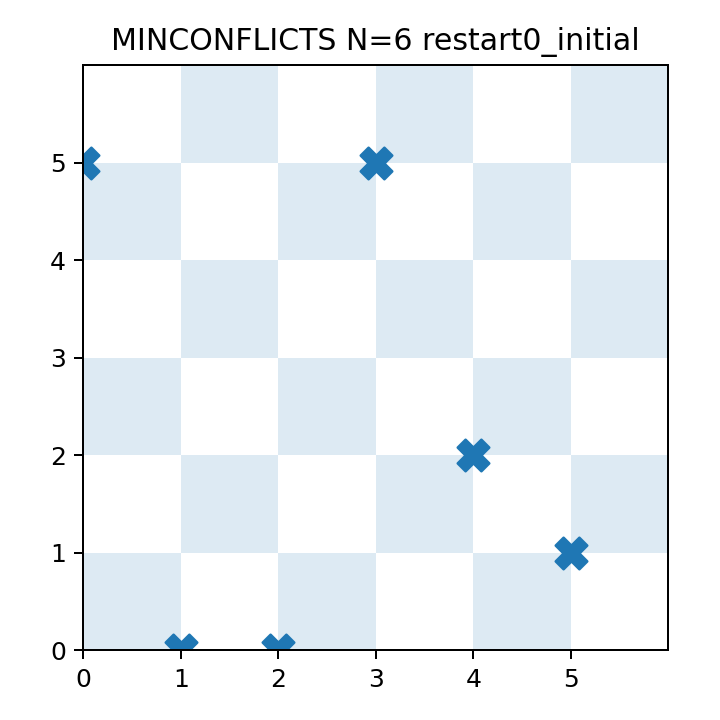
\includegraphics[width=\linewidth]{\figdir/n6_initial.png}
    \caption{Initial}
  \end{subfigure}\hfill
  \begin{subfigure}{.31\linewidth}
    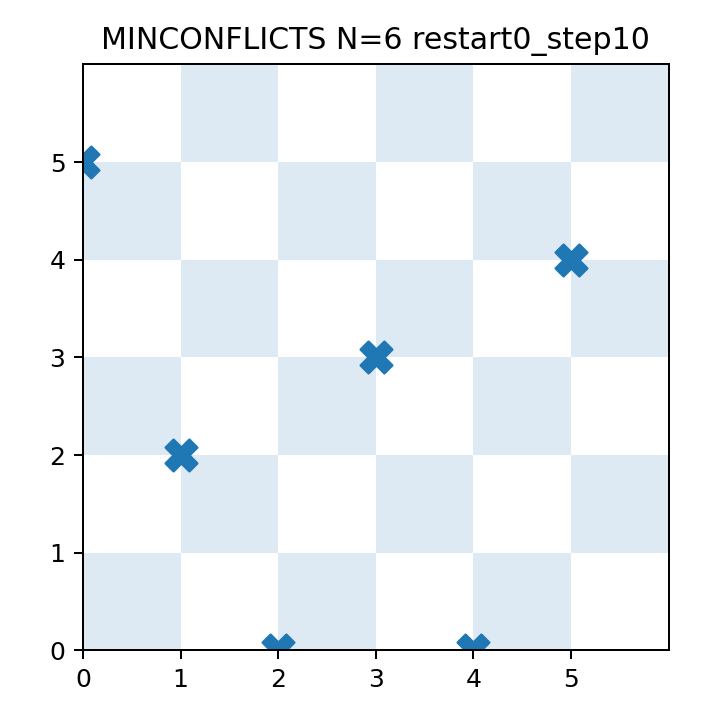
\includegraphics[width=\linewidth]{\figdir/n6_step1.png}
    \caption{Step 1}
  \end{subfigure}\hfill
  \begin{subfigure}{.31\linewidth}
    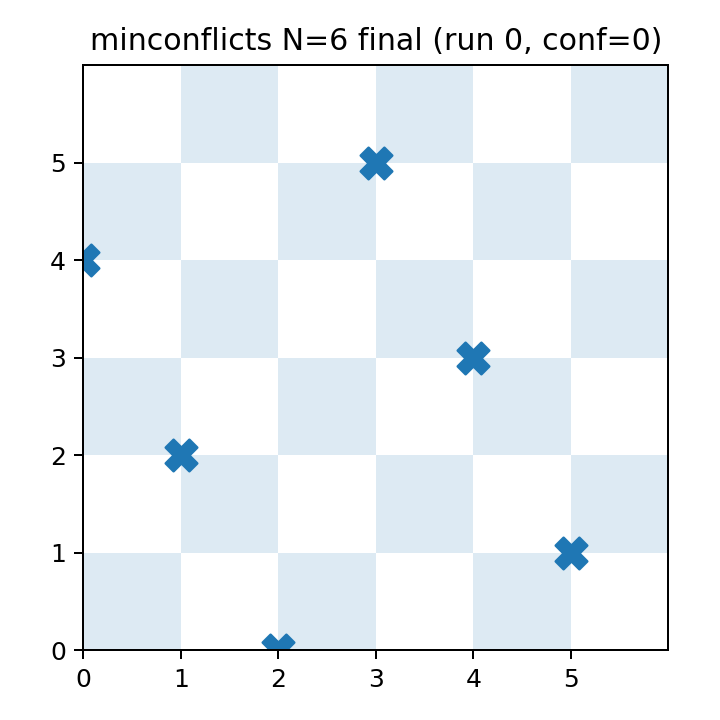
\includegraphics[width=\linewidth]{\figdir/n6_final.png}
    \caption{Final}
  \end{subfigure}
  \caption{N=6 snapshots (Min-Conflicts shown). Early moves reduce row/diagonal clashes as queens relocate to less contested rows.}
\end{figure}
\FloatBarrier

\subsection{Final Solutions (N=8,10,12)}
\begin{figure}[H]\centering
  \begin{subfigure}{.48\linewidth}
    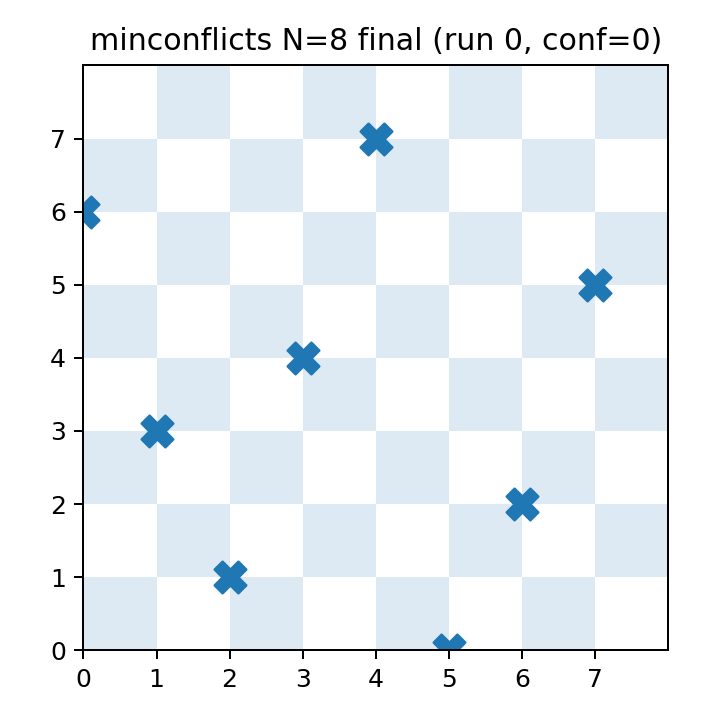
\includegraphics[width=\linewidth]{\figdir/minconflicts_n8_final.png}
    \caption{Min-Conflicts, N=8}
  \end{subfigure}\hfill
  \begin{subfigure}{.48\linewidth}
    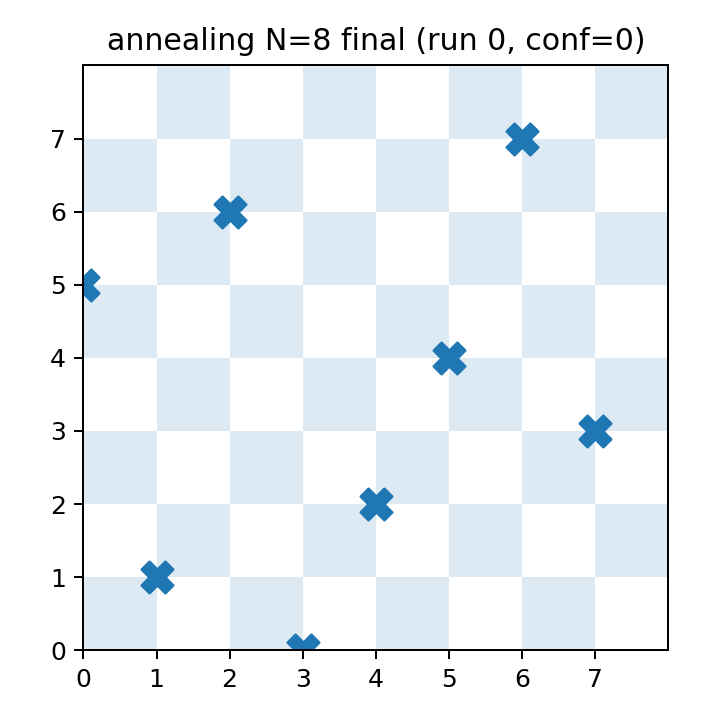
\includegraphics[width=\linewidth]{\figdir/annealing_n8_final.png}
    \caption{Annealing, N=8}
  \end{subfigure}
  \caption{Representative final boards for N=8.}
\end{figure}

\begin{figure}[H]\centering
  \begin{subfigure}{.48\linewidth}
    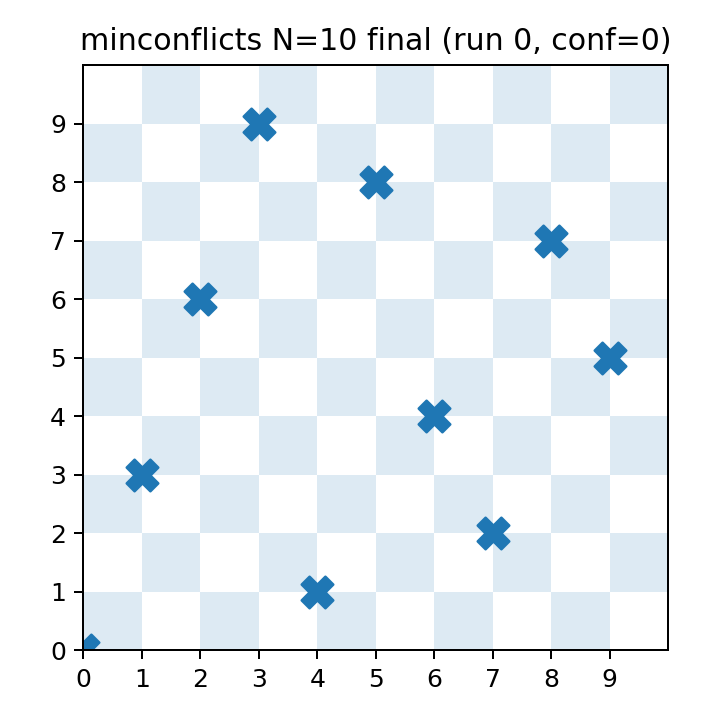
\includegraphics[width=\linewidth]{\figdir/minconflicts_n10_final.png}
    \caption{Min-Conflicts, N=10}
  \end{subfigure}\hfill
  \begin{subfigure}{.48\linewidth}
    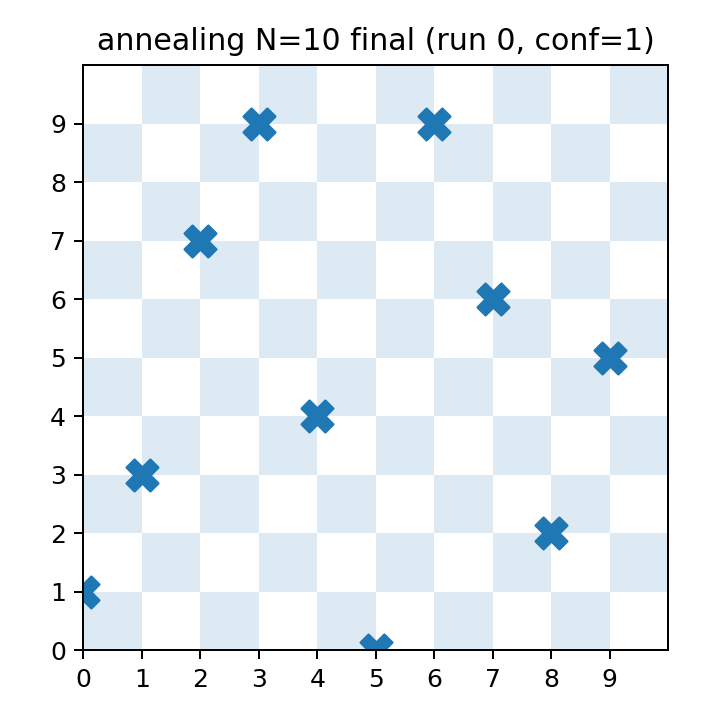
\includegraphics[width=\linewidth]{\figdir/annealing_n10_final.png}
    \caption{Annealing, N=10}
  \end{subfigure}
  \caption{Representative final boards for N=10.}
\end{figure}

\begin{figure}[H]\centering
  \begin{subfigure}{.48\linewidth}
    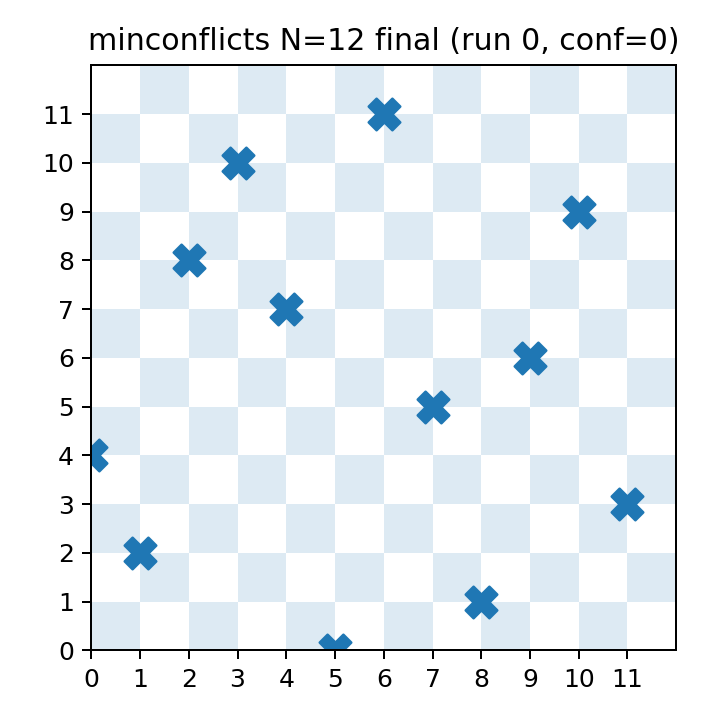
\includegraphics[width=\linewidth]{\figdir/minconflicts_n12_final.png}
    \caption{Min-Conflicts, N=12}
  \end{subfigure}\hfill
  \begin{subfigure}{.48\linewidth}
    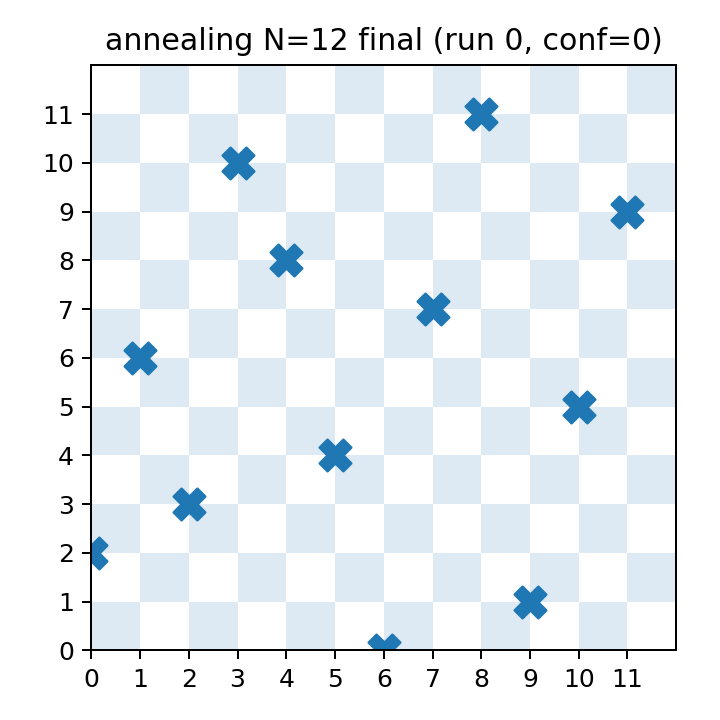
\includegraphics[width=\linewidth]{\figdir/annealing_n12_final.png}
    \caption{Annealing, N=12}
  \end{subfigure}
  \caption{Representative final boards for N=12.}
\end{figure}
\FloatBarrier

\subsection{Quantitative Results}
\input{../results/tables/nqueens_agg.tex}

\subsection{Implementation Details}
States are 1D arrays of rows per column; cost $h$ counts attacking pairs. Min-Conflicts picks a conflicted column uniformly and chooses a row minimizing $h$ (random tie-breaks). We use a step cap of 10k and up to 100 restarts. Annealing uses $(T_0{=}1.0,\ \alpha{=}0.995,\ T_{\min}{=}10^{-3})$ and a 100k step cap.

\subsection{Threats to Validity}
Reported times are single-run wall-clock on the stated machine and may vary across hardware. Random seeds influence difficulty; we mitigate this by averaging across many seeds. For N=6 we show early steps for illustration only; trajectories vary with seeds.

\subsection*{Key Code Excerpts}

\paragraph{Conflict (cost) function.}
\begin{lstlisting}[style=mypython,caption={Number of attacking pairs},label={lst:conflicts}]
def conflicts(state):
    n = len(state)
    c = 0
    for i in range(n):
        for j in range(i + 1, n):
            if state[i] == state[j] or abs(state[i] - state[j]) == abs(i - j):
                c += 1
    return c
\end{lstlisting}

\paragraph{Min-Conflicts step (choose conflicted column, move to best row).}
\begin{lstlisting}[style=mypython,caption={Min-Conflicts local repair step},label={lst:minc-step}]
conflicted = _conflicted_columns(state)
col = rng.choice(conflicted)
state[col] = _best_row_for_col(state, col, rng)
\end{lstlisting}

\paragraph{Simulated annealing acceptance (occasionally accept uphill moves).}
\begin{lstlisting}[style=mypython,caption={Annealing acceptance rule},label={lst:anneal-accept}]
delta = new_c - cur_c
if delta <= 0 or rng.random() < math.exp(-delta / T):
    cur_c = new_c   # accept move
else:
    state[col] = old_row  # reject move
T *= alpha
\end{lstlisting}

\subsection{Discussion}
On these sizes, Min-Conflicts typically converged rapidly due to the problem's local-repair structure; failures arise from plateaus/cycles and are mitigated by restarts. Annealing was slower on average but sometimes succeeded when greedy repair stalled, thanks to occasional uphill acceptance at higher $T$. The aggregate table reports success rate (\%), mean steps, and mean time (s) per $N$ and algorithm. Practical levers include the Min-Conflicts step cap/restart count and the annealing schedule $(T_0,\alpha)$; gentler cooling (larger $\alpha$) improves success at a runtime cost.

\section{Learning: IRIS Classification}

\subsection{Setup}
We use the Moodle dataset \verb|iris.arff| (150 samples, 3 classes). All models share a stratified split (\verb|test_size=0.3|, \verb|seed=123|). We compare all four features vs.\ two features (petal length/width). Metrics: accuracy, macro precision/recall/F1; timing via \verb|time.perf_counter()|.

\subsection{Models and Training Details}
We parse \verb|iris.arff|, decode the nominal \verb|class| labels, and keep the original ARFF feature names (sepallength, sepalwidth, petallength, petalwidth). To guarantee comparability, we cache the \emph{same} stratified split indices and reuse them for all models and for both 4-feature and 2-feature settings. We train:
\begin{itemize}
  \item \textbf{k-NN} (k=5), applied after standardization.
  \item \textbf{Decision Tree} with default settings (random state 123).
  \item \textbf{MLP (backprop)}: one hidden layer with $h\in\{4,8,16,32\}$ using \texttt{MLPClassifier}; inputs are standardized; iteration cap chosen to converge on IRIS.
\end{itemize}
Confusion matrices and metrics are computed on the held-out test set; wall-clock training times are recorded.

\subsection*{Key Code Excerpts (IRIS)}

\paragraph{Data loader (ARFF).}
\begin{lstlisting}[style=mypython,caption={Load IRIS from ARFF and optionally keep two petal features},label={lst:iris-loader}]
from scipy.io import arff
import pandas as pd
import numpy as np

def load_iris(arff_path, two_features=False):
    data, meta = arff.loadarff(arff_path)
    df = pd.DataFrame(data)
    y = df["class"].apply(lambda v: v.decode() if isinstance(v,(bytes,bytearray)) else v).to_numpy()
    X = df.drop(columns=["class"]).to_numpy(dtype=float)
    feature_names = [c for c in df.columns if c != "class"]
    if two_features:
        cols = ["petallength", "petalwidth"]
        idx = [feature_names.index(c) for c in cols]
        X = X[:, idx]
        feature_names = [feature_names[i] for i in idx]
    return X, y, feature_names
\end{lstlisting}

\paragraph{Split caching (same train and test for every model).}
\begin{lstlisting}[style=mypython,caption={Stratified split with cached indices for reproducibility},label={lst:iris-split}]
import os, json
import numpy as np
from sklearn.model_selection import train_test_split

def stratified_cached_split(X, y, seed=123, test_size=0.3, cache="results/logs/iris_split_idx.json"):
    key = f"seed{seed}_ts{test_size}"
    try:
        d = json.load(open(cache))
        idx_tr = np.array(d[key]["train"], dtype=int)
        idx_te = np.array(d[key]["test"], dtype=int)
    except Exception:
        idx = np.arange(len(y))
        _, _, _, _, idx_tr, idx_te = train_test_split(
            X, y, idx, test_size=test_size, random_state=seed, stratify=y
        )
        os.makedirs(os.path.dirname(cache), exist_ok=True)
        d = {} if not os.path.exists(cache) else json.load(open(cache))
        d[key] = {"train": idx_tr.tolist(), "test": idx_te.tolist()}
        json.dump(d, open(cache, "w"), indent=2)
    return idx_tr, idx_te
\end{lstlisting}

\paragraph{Models (k-NN, Decision Tree, MLP with backprop).}
\begin{lstlisting}[style=mypython,caption={Model definitions with standardization where useful},label={lst:iris-models}]
from sklearn.pipeline import make_pipeline
from sklearn.preprocessing import StandardScaler
from sklearn.neighbors import KNeighborsClassifier
from sklearn.tree import DecisionTreeClassifier
from sklearn.neural_network import MLPClassifier

knn = make_pipeline(StandardScaler(), KNeighborsClassifier(n_neighbors=5))
dt  = DecisionTreeClassifier(random_state=123)
mlp = make_pipeline(StandardScaler(),
                    MLPClassifier(hidden_layer_sizes=(8,),
                                  solver="lbfgs",
                                  max_iter=2000,
                                  random_state=123))
\end{lstlisting}

\paragraph{Metrics and confusion matrix plotting.}
\begin{lstlisting}[style=mypython,caption={Metrics and confusion matrix utility},label={lst:iris-metrics}]
import matplotlib.pyplot as plt
from sklearn.metrics import (accuracy_score, precision_recall_fscore_support,
                             confusion_matrix, ConfusionMatrixDisplay)

def evaluate(y_true, y_pred):
    acc = accuracy_score(y_true, y_pred)
    prec, rec, f1, _ = precision_recall_fscore_support(
        y_true, y_pred, average="macro", zero_division=0
    )
    return acc, prec, rec, f1

def plot_cm(y_true, y_pred, labels, title, out_png):
    cm = confusion_matrix(y_true, y_pred, labels=labels)
    disp = ConfusionMatrixDisplay(confusion_matrix=cm, display_labels=labels)
    fig, ax = plt.subplots(figsize=(4, 4))
    disp.plot(ax=ax, values_format="d", colorbar=False)
    ax.set_title(title)
    fig.tight_layout()
    fig.savefig(out_png, dpi=180)
    plt.close(fig)
\end{lstlisting}

\subsection{Confusion Matrices (2 features)}
\begin{figure}[H]\centering
  \begin{subfigure}{.32\linewidth}
    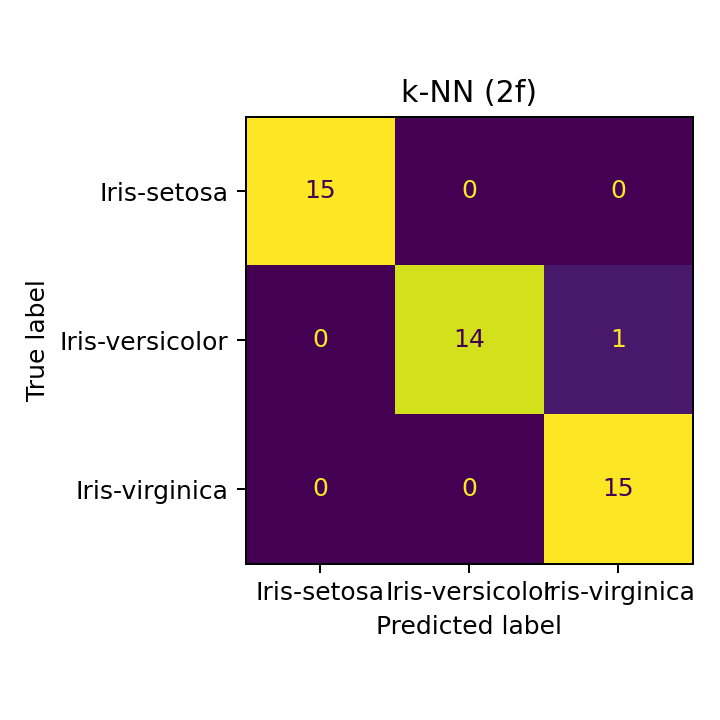
\includegraphics[width=\linewidth]{\figdir/confusion_matrix_knn_2f.png}
    \caption{k-NN}
  \end{subfigure}\hfill
  \begin{subfigure}{.32\linewidth}
    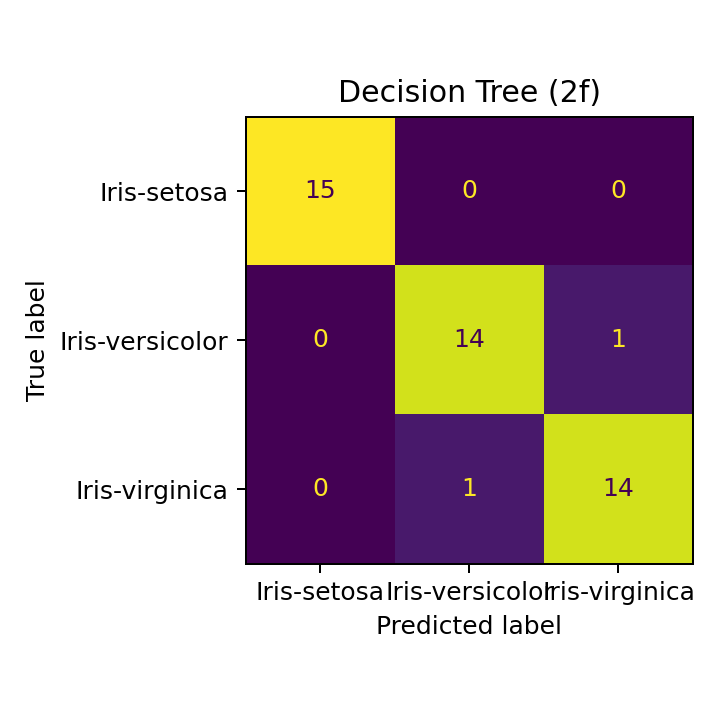
\includegraphics[width=\linewidth]{\figdir/confusion_matrix_decision_tree_2f.png}
    \caption{Decision Tree}
  \end{subfigure}\hfill
  \begin{subfigure}{.32\linewidth}
    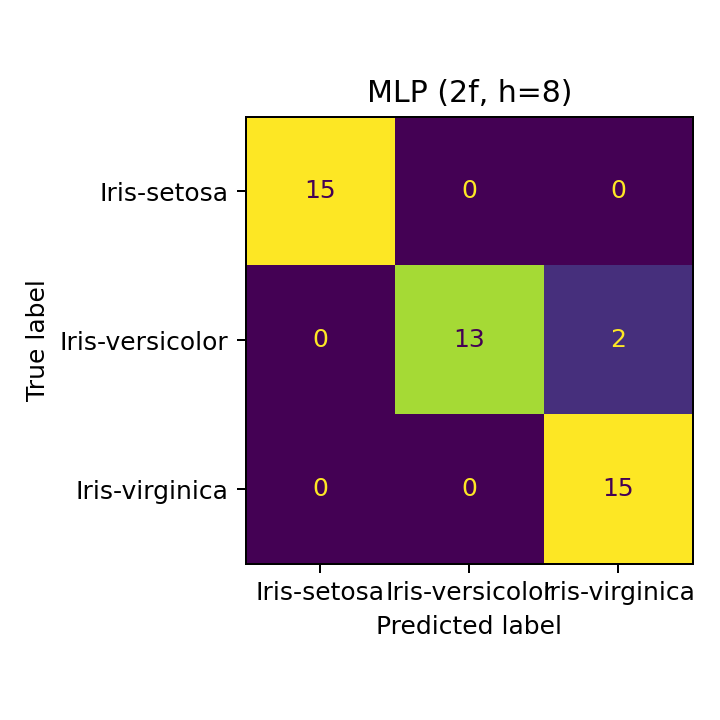
\includegraphics[width=\linewidth]{\figdir/confusion_matrix_mlp_2f.png}
    \caption{MLP (backprop)}
  \end{subfigure}
  \caption{IRIS two-feature classification (petal length/width).}
\end{figure}

\subsection{Confusion Matrices (4 features)}
\begin{figure}[H]\centering
  \begin{subfigure}{.32\linewidth}
    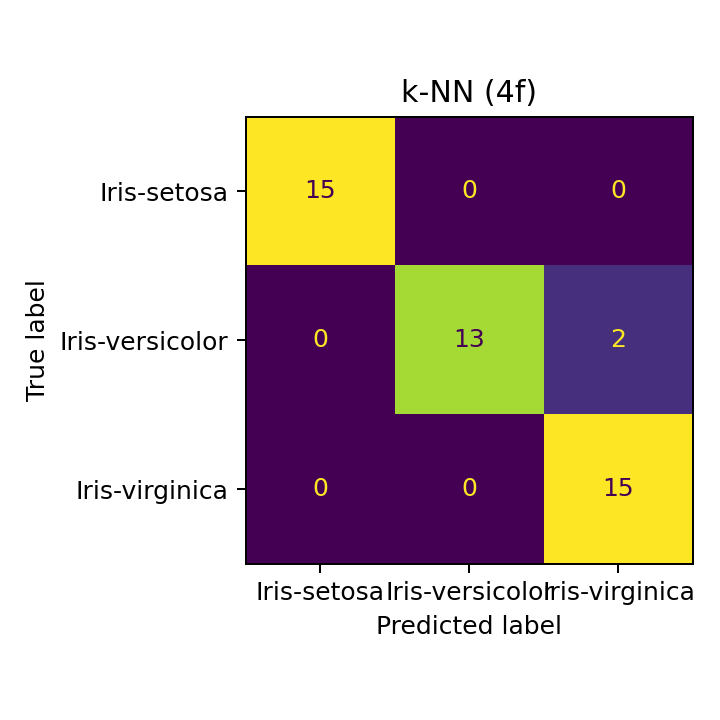
\includegraphics[width=\linewidth]{../results/figures/confusion_matrix_knn_4f.png}
    \caption{k-NN}
  \end{subfigure}\hfill
  \begin{subfigure}{.32\linewidth}
    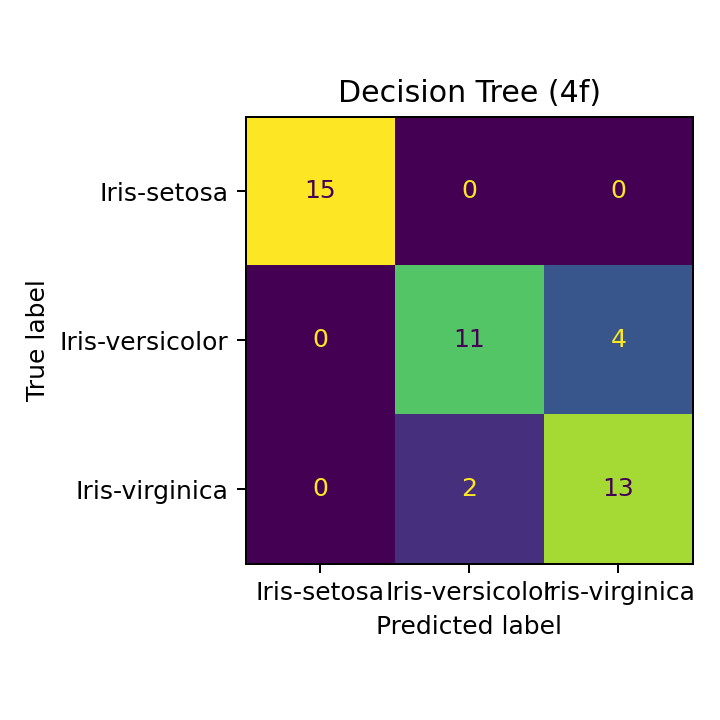
\includegraphics[width=\linewidth]{../results/figures/confusion_matrix_decision_tree_4f.png}
    \caption{Decision Tree}
  \end{subfigure}\hfill
  \begin{subfigure}{.32\linewidth}
    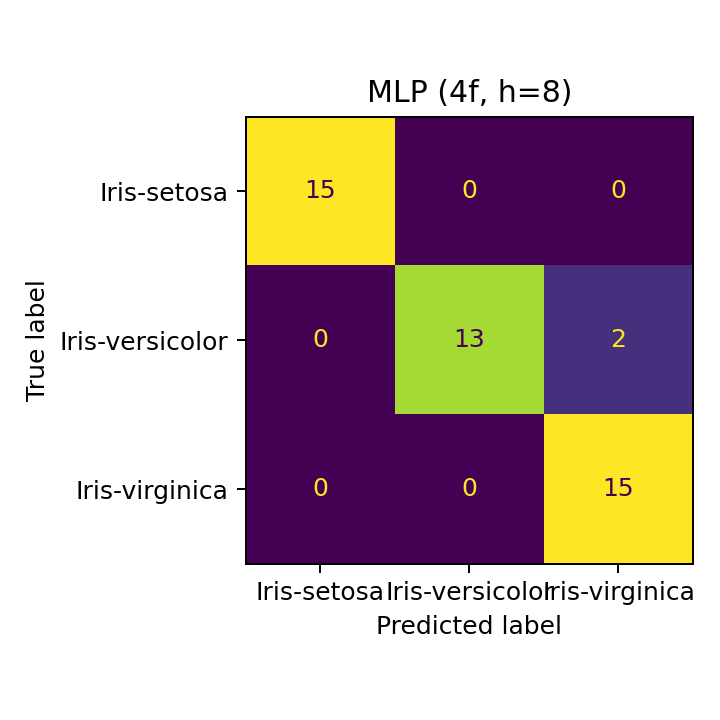
\includegraphics[width=\linewidth]{../results/figures/confusion_matrix_mlp_4f.png}
    \caption{MLP (backprop)}
  \end{subfigure}
  \caption{IRIS four-feature classification.}
\end{figure}

\subsection{Quantitative Results}
\input{../results/tables/iris_agg.tex}

\subsection{NN Topology and Discussion}
We varied the NN hidden units ($h\in\{4,8,16,32\}$) and selected $h=8$ as a good trade-off between accuracy and time on this small dataset. All models classify \emph{setosa} perfectly; most errors occur between \emph{versicolor} and \emph{virginica}. Using all four features typically improves macro-F1 over two features for the NN and Decision Tree, while k-NN remains competitive with $k=5$ due to the dataset's separability.

\subsection{NN Topology Sweep}
\input{../results/tables/iris_mlp_sweep.tex}

\section*{Conclusion}
\textbf{Local Search (N-Queens).} Min-Conflicts rapidly found solutions on $N\le12$, with restarts mitigating plateaus; Simulated Annealing was slower but occasionally escaped local minima when greedy repair stalled. \textbf{IRIS Classification.} All models separated \emph{setosa} perfectly; most confusion occurred between \emph{versicolor} and \emph{virginica}. Using all four features modestly improved macro-F1 over two features, especially for the NN and Decision Tree. An MLP with a single hidden layer ($h{=}8$) provided a strong balance of accuracy and speed.

\begin{thebibliography}{9}
\bibitem{uci-iris}
Dua, D. and Graff, C. (2019). \emph{UCI Machine Learning Repository: Iris Data Set}. \url{https://archive.ics.uci.edu/ml/datasets/iris}. (Accessed via Moodle \texttt{iris.arff}.)

\bibitem{sklearn}
Pedregosa, F. et al. (2011). Scikit-learn: Machine Learning in Python. \emph{JMLR}, 12:2825--2830. \url{https://scikit-learn.org/}

\bibitem{russell-norvig}
Russell, S. and Norvig, P. (2010). \emph{Artificial Intelligence: A Modern Approach} (3rd ed.). (Background on local search and Min-Conflicts.)
\end{thebibliography}

\end{document}
